\documentclass{article}
\usepackage{arxiv}

\usepackage[utf8]{inputenc}
\usepackage[english, russian]{babel}
\usepackage[T1]{fontenc}
\usepackage{url}
\usepackage{booktabs}
\usepackage{amsfonts}
\usepackage{nicefrac}
\usepackage{microtype}
\usepackage{lipsum}
\usepackage{graphicx}
\usepackage{natbib}
\usepackage{doi}
\usepackage{hyperref}

\usepackage{listings}


\usepackage{euscript}	 % Шрифт Евклид
\usepackage{mathrsfs} % Красивый матшрифт

%% Перенос знаков в формулах (по Львовскому)
\newcommand*{\hm}[1]{#1\nobreak\discretionary{}
{\hbox{$\mathsurround=0pt #1$}}{}}

%%% Работа с картинками
\usepackage{graphicx}  % Для вставки рисунков
% \graphicspath{{images/}{images2/}}  % папки с картинками
\setlength\fboxsep{5pt} % Отступ рамки \fbox{} от рисунка
\setlength\fboxrule{5pt} % Толщина линий рамки \fbox{}
\usepackage{wrapfig} % Обтекание рисунков и таблиц текстом

%%% Работа с таблицами
\usepackage{array,tabularx,tabulary,booktabs} % Дополнительная работа с таблицами
\usepackage{longtable}  % Длинные таблицы
\usepackage{multirow} % Слияние строк в таблице




\title{Flood risk predictions via machine learning methods}

\author{ Vladislav Pyzh	\\
	MIPT\\
	Moscow, Russia \\
	\texttt{pyzh.va@phystech.edu} \\
	%% examples of more authors
% 	\And
% 	Yuriy Maximov \\
% 	Research Center in Artificial Intelligence
% Skoltech\\
% 	\\
% 	\texttt{} \\
	%% \AND
	%% Coauthor \\
	%% Affiliation \\
	%% Address \\
	%% \texttt{email} \\
	%% \And
	%% Coauthor \\
	%% Affiliation \\
	%% Address \\
	%% \texttt{email} \\
	%% \And
	%% Coauthor \\
	%% Affiliation \\
	%% Address \\
	%% \texttt{email} \\
}
\date{}

\renewcommand{\shorttitle}{\textit{arXiv} Template}

%%% Add PDF metadata to help others organize their library
%%% Once the PDF is generated, you can check the metadata with
%%% $ pdfinfo template.pdf
\hypersetup{
pdftitle={A template for the arxiv style},
pdfsubject={q-bio.NC, q-bio.QM},
pdfauthor={David S.~Hippocampus, Elias D.~Striatum},
pdfkeywords={First keyword, Second keyword, More},
}

\begin{document}
\maketitle

% \begin{abstract}
% В данной работе рассматривается задача предсказания экстремальных климатических явлений, а именно наводнений. Прогнозирование осуществляется в краткосрочном диапозоне для стационарных временных рядов и в длинном диапозоне для нестационарных рядов. Существенной особенностью данной задачи является необходимость предсказывания экстремальных значений с высокой точностью, тогда как точность предсказаний малых изменений не представляет интерес.
% \end{abstract}

\begin{abstract}
    In this work we observe extreme weather condition predictions, we particularly focus on floods. We make predictions in short-term periods assuming we have stationary time series and in long-term periods assuming we have not stationary time series. The main feature of this problem is that we want to predict extreme values with high accuracy, whether prediction of low values is not very sufficient.  
\end{abstract}

\section{Introduction}
Extreme weather events can lead to high economic costs thus it is preferable to predict them. Main goal of our work is to develop model, which can be used in practice to predict these events. Formally speaking we are solving classification task on geo-spatial time series. This task contains two different situations: predictions on stationary time series in short-term periods and not stationary in long-term periods. We assume that weather in period shorter than 5-10 years does not have common trend, so we analyze stationary time series. On the other hand in long run we can assume that weather coditions are likely to change, so we have to take into account that this time series can be not stationary. The main issue on this problem is that events that we can interpret as positive object in our classification task are extremely rare. Speaking more precisely from 1980's \href{http://www.overleaf.com}{there were} less than 10 big flood in state California. Thus we use several techniques like SMOTE and under-sampling. Also we should notice that prediction model has to provide low recall, because it is important, not to skip events in this case.  Another goal of our work is combining state-of-the-art solutions to improve current result in sphere. We base our decision on works ~\cite{put link here} and ~\cite{put link here}. We implement (Подробнее описать какие state-of-the-art методы мы хотим использовать в работе, в чем заключается её новизна?)

\section{Problem statement}
As mentioned before we solve classification task. Let $Tr = (X_{tr}, y_{tr})$ be our train set, $\widehat{y}(Tr)$ our model, thus we solve optimisation problem 

$$y^* = arg \min\limits_{\widehat{y}} \sum \limits _{(X_{ts}, y_{ts})} L(\widehat{y}(X_{tr}, y_{tr}), y_{ts})$$

Lets formally describe what actually means that our model has to achieve low recall (На этой стадии пока не обозначили какой результат именно хотели получить)

\section{Planning Experiment}
During experiment we aimed to achieve model hyperparameters that improve our known results. Earlier we reached these results:

\begin{wraptable}{r}{0.5\linewidth}
		\begin{tabular}{|c|c|c|}
			\hline
			Model & SVM and SMOTE & SVM and RU \\ \hline
			precision &  0.151 & 0.147 \\ \hline
			recall & 0.367 & 0.533  \\ \hline
			accuracy & 0.925 & 0.901  \\ \hline
			F1-score &  0.214 & 0.230 \\ \hline
		\end{tabular}
		\caption{Our previous results}
\end{wraptable}We use combine linear models, different variations of boosting, random forest and svm with techniques which solves extreme values rarity. Overall we can describe our pipeline: split our data on test and train, use some algorithm to solve class disbalance problem in train, use grid search to tune our model parameters via cross validation on train, measure our prediction accuracy.

In our experiment we use meteorological data across California from  1980-01-01 till 2019-12-31 only in winter. We have 8 features, described below:
\begin{itemize}
    \item h500 – 500 hPa geopotential height 
    \item ivt - integrated vapor transport 
    \item qv2m- 2-meter specific humidity
    \item slp - sea level pressure 
    \item tpw -total precipitable water
    \item uqv – zonal component of integrated vapor transport
    \item vqv – meridional component of integrated vapor transport
    \item w500 – 500 hpa vertical pressure velocity
\end{itemize}
Thus in this experiment we compare a well-known machine learning techniques with our data. Since main goal of out work is to predict events, most effective models we use in Time Series analyze with some extra features like shifted features, mean values and so on.

Final result of this experiment is pivot table, where we can easily compare models.



\section{Run basic code and preliminary results}
Below we give an example of basic experiment code. Unfortunately google colab resources are too restricted, so now we stucked on this stage (перезапущу еще на персональном компьютере, должно получиться). 

\begin{lstlisting}
search_cat = RandomizedSearchCV(
      estimator=CatBoostClasifier(verbose=0),
      param_distributions={
          "reg_lambda": np.logspace(-4, 0, 30),
          "n_estimators" : np.arange(450, 1000, 20),
          "learning_rate" : np.linspace(0.001, 0.02, 40),
          "max_depth": np.arange(4, 20)
      },
      scoring='recall',
      n_iter=25,
      n_jobs=-1
)
search_cat.fit(X_train_smote, y_train_smote)
\end{lstlisting}

Nevertheless we can obtain example of final result without RandomizedSearchCV on default CatBoostClassifier parameters.

\begin{itemize}
    \item Accuracy =  0.948
    \item Precision =  0.167
    \item Recall =  0.368
    \item F1 Score =  0.230
\end{itemize}


\begin{wraptable}{r}{0.5\linewidth}
		\begin{tabular}{|c|c|}
			\hline
			True Negative = 848 & False Positive = 35 \\ \hline
			False Negative = 12 &  True Positive = 7 \\ \hline
		\end{tabular}
		\caption{Confusion matrix}
\end{wraptable}For this experiment we also have confusion matrix.

\section{Experiment description }
During this experiment we tested CatBoost, SVC with linear and rbf kernels, RandomForest and Logistic regression. To nullify big class disbalance we used SMOTE and RandomUndersampling. We used geo-spatial dataset with data across west coast of the United States, we illustrated it here. It has approximately 400 rows about every point in winter only.
\begin{center}
\caption{Dataset points on USA map}
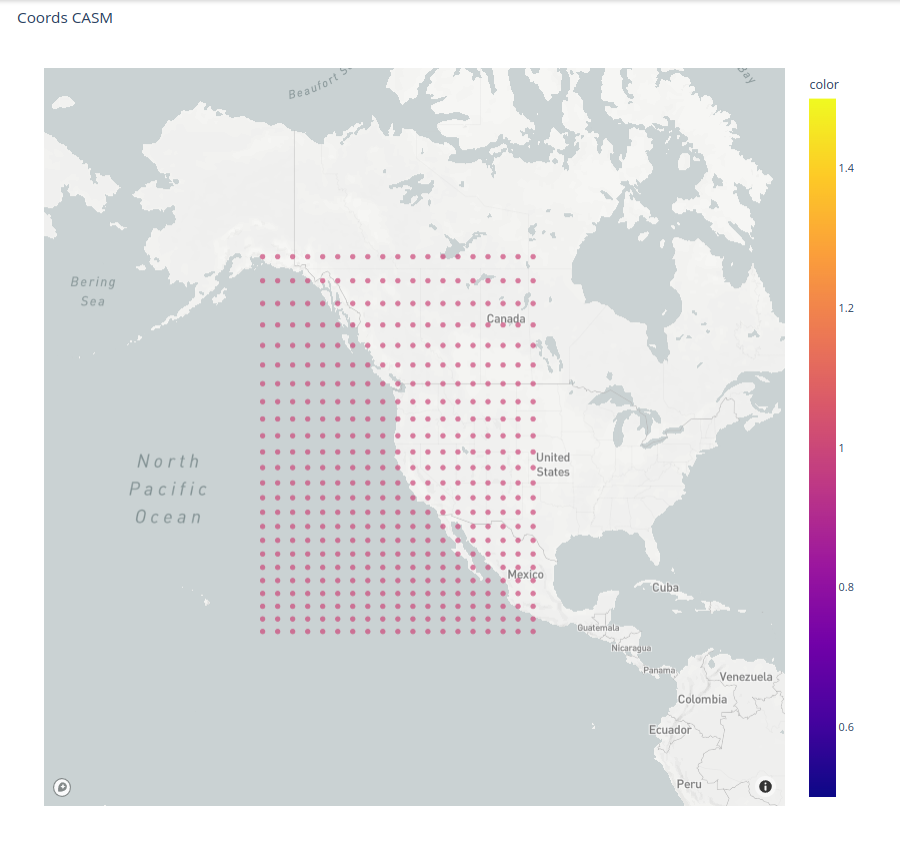
\includegraphics[width=0.8\textwidth]{map.png}
\end{center}




\section{Experiment results}
\begin{center}
\caption{Dataset points on USA map}
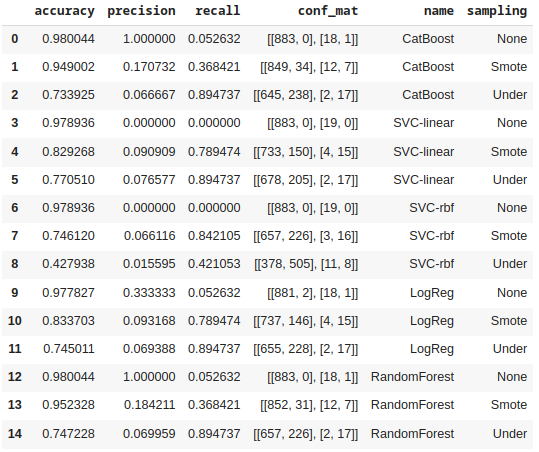
\includegraphics[width=0.8\textwidth]{pivot_table.png}
\end{center}

\section{Plot list}
In this paper we use these plots: 
\begin{itemize}
    \item Data visualisation
    \item Results pivot table
    \item (Consider using this ??) Results comparation with lines?
    \item (Code is not done yet) DL techonologies visualistion
\end{itemize}

\section{Theoretical description}
Let's consider our extreme event as high percentile of precipitation in area. As we want to predict flood risks in California our target event on whole dataset is extreme events only in California. Formaly speaking we work with spatial series and we can describe our problem so:
$$
y_t = \sum\limits^n_{i=1} F(Y_{t-i}) + E_t +\epsilon_t
$$
Here n denotes amount of previous significant events that contribute in our estimation, $Y_{t-i}$ is a spatial tensor of these events containing eight parameters (thus it has size (8, 24, 19)). $F$ is an implicit dependence, $epsilon$ is a random noise and $E$ is an error . Our aim is to choose machine learning methods that minimize error suggesting that noise has a zero mean value.  
 
\section{Error analysis}
We made a basic experiment with a convolution neural network. As loss criterion we use cross entropy function. Base on this graphics we conclude that we can improve our quality by increasing epochs, which is next goal of this work
\begin{center}
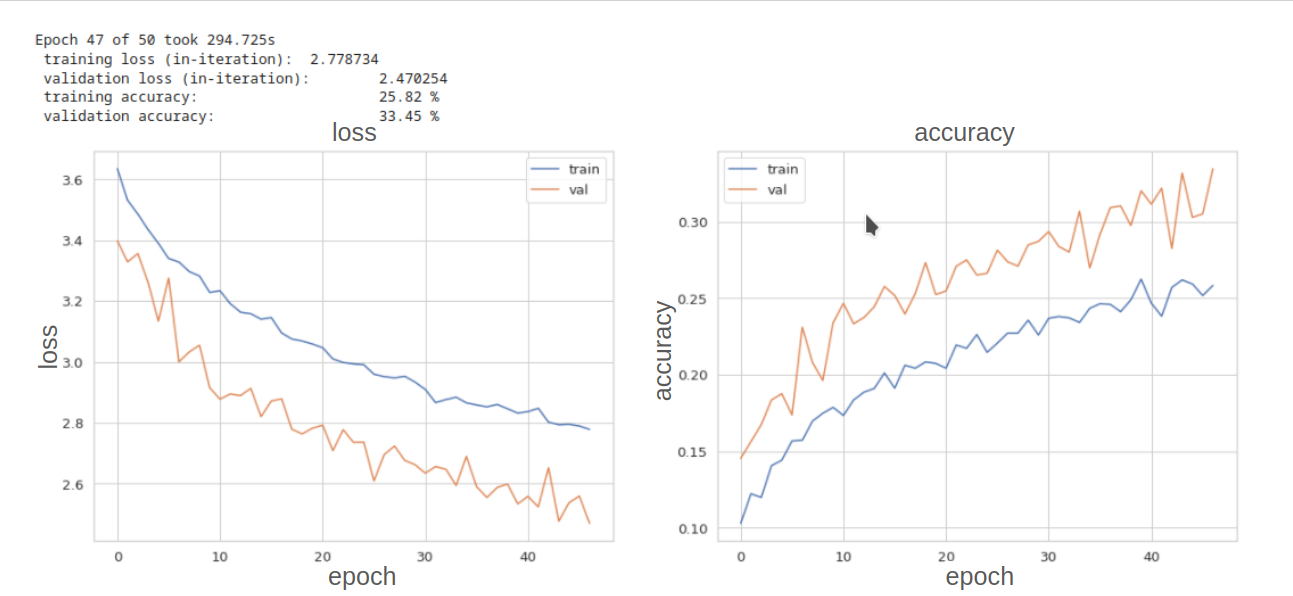
\includegraphics[width=1\textwidth]{Loss plots.png}
\end{center}

\end{document}